\section{Implementation}

In this section some implementation details will be given for the animations and effects.

\subsection{Environment}
An important part in the user experience with mixed and virtual reality plays the virtual environment. Here a combination of a skybox and an environment 3D-model was used to get the most out of the V2C cave regarding to immersion. The skybox image was rendered using an HDRI image and a self written hdri to image converter in Blender 3D.

\begin{figure}[!ht]
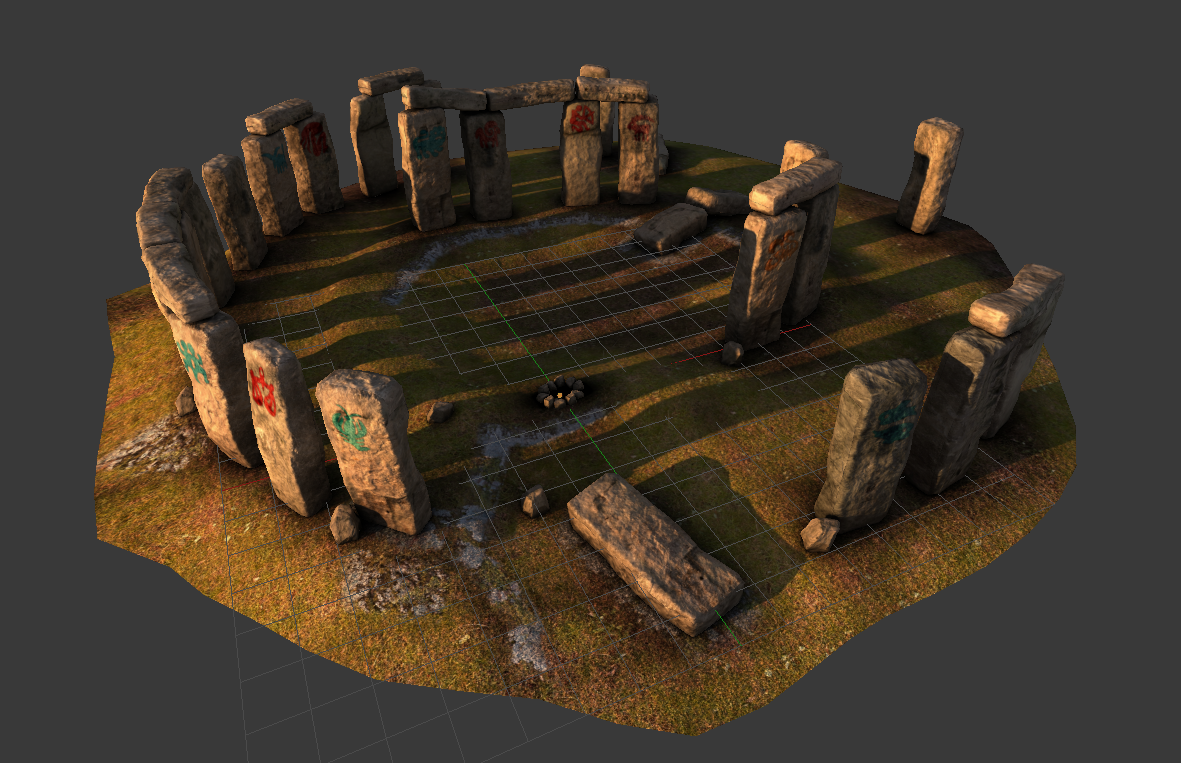
\includegraphics[width=0.4\textwidth]{pictures/stonehenge.png}
\caption{Stonehenge by ruslans3d is licensed under CC Attribution https://sketchfab.com/models/37cfc2bb99944703b5d57ea281030ca6}
\end{figure}

\begin{figure}[!ht]
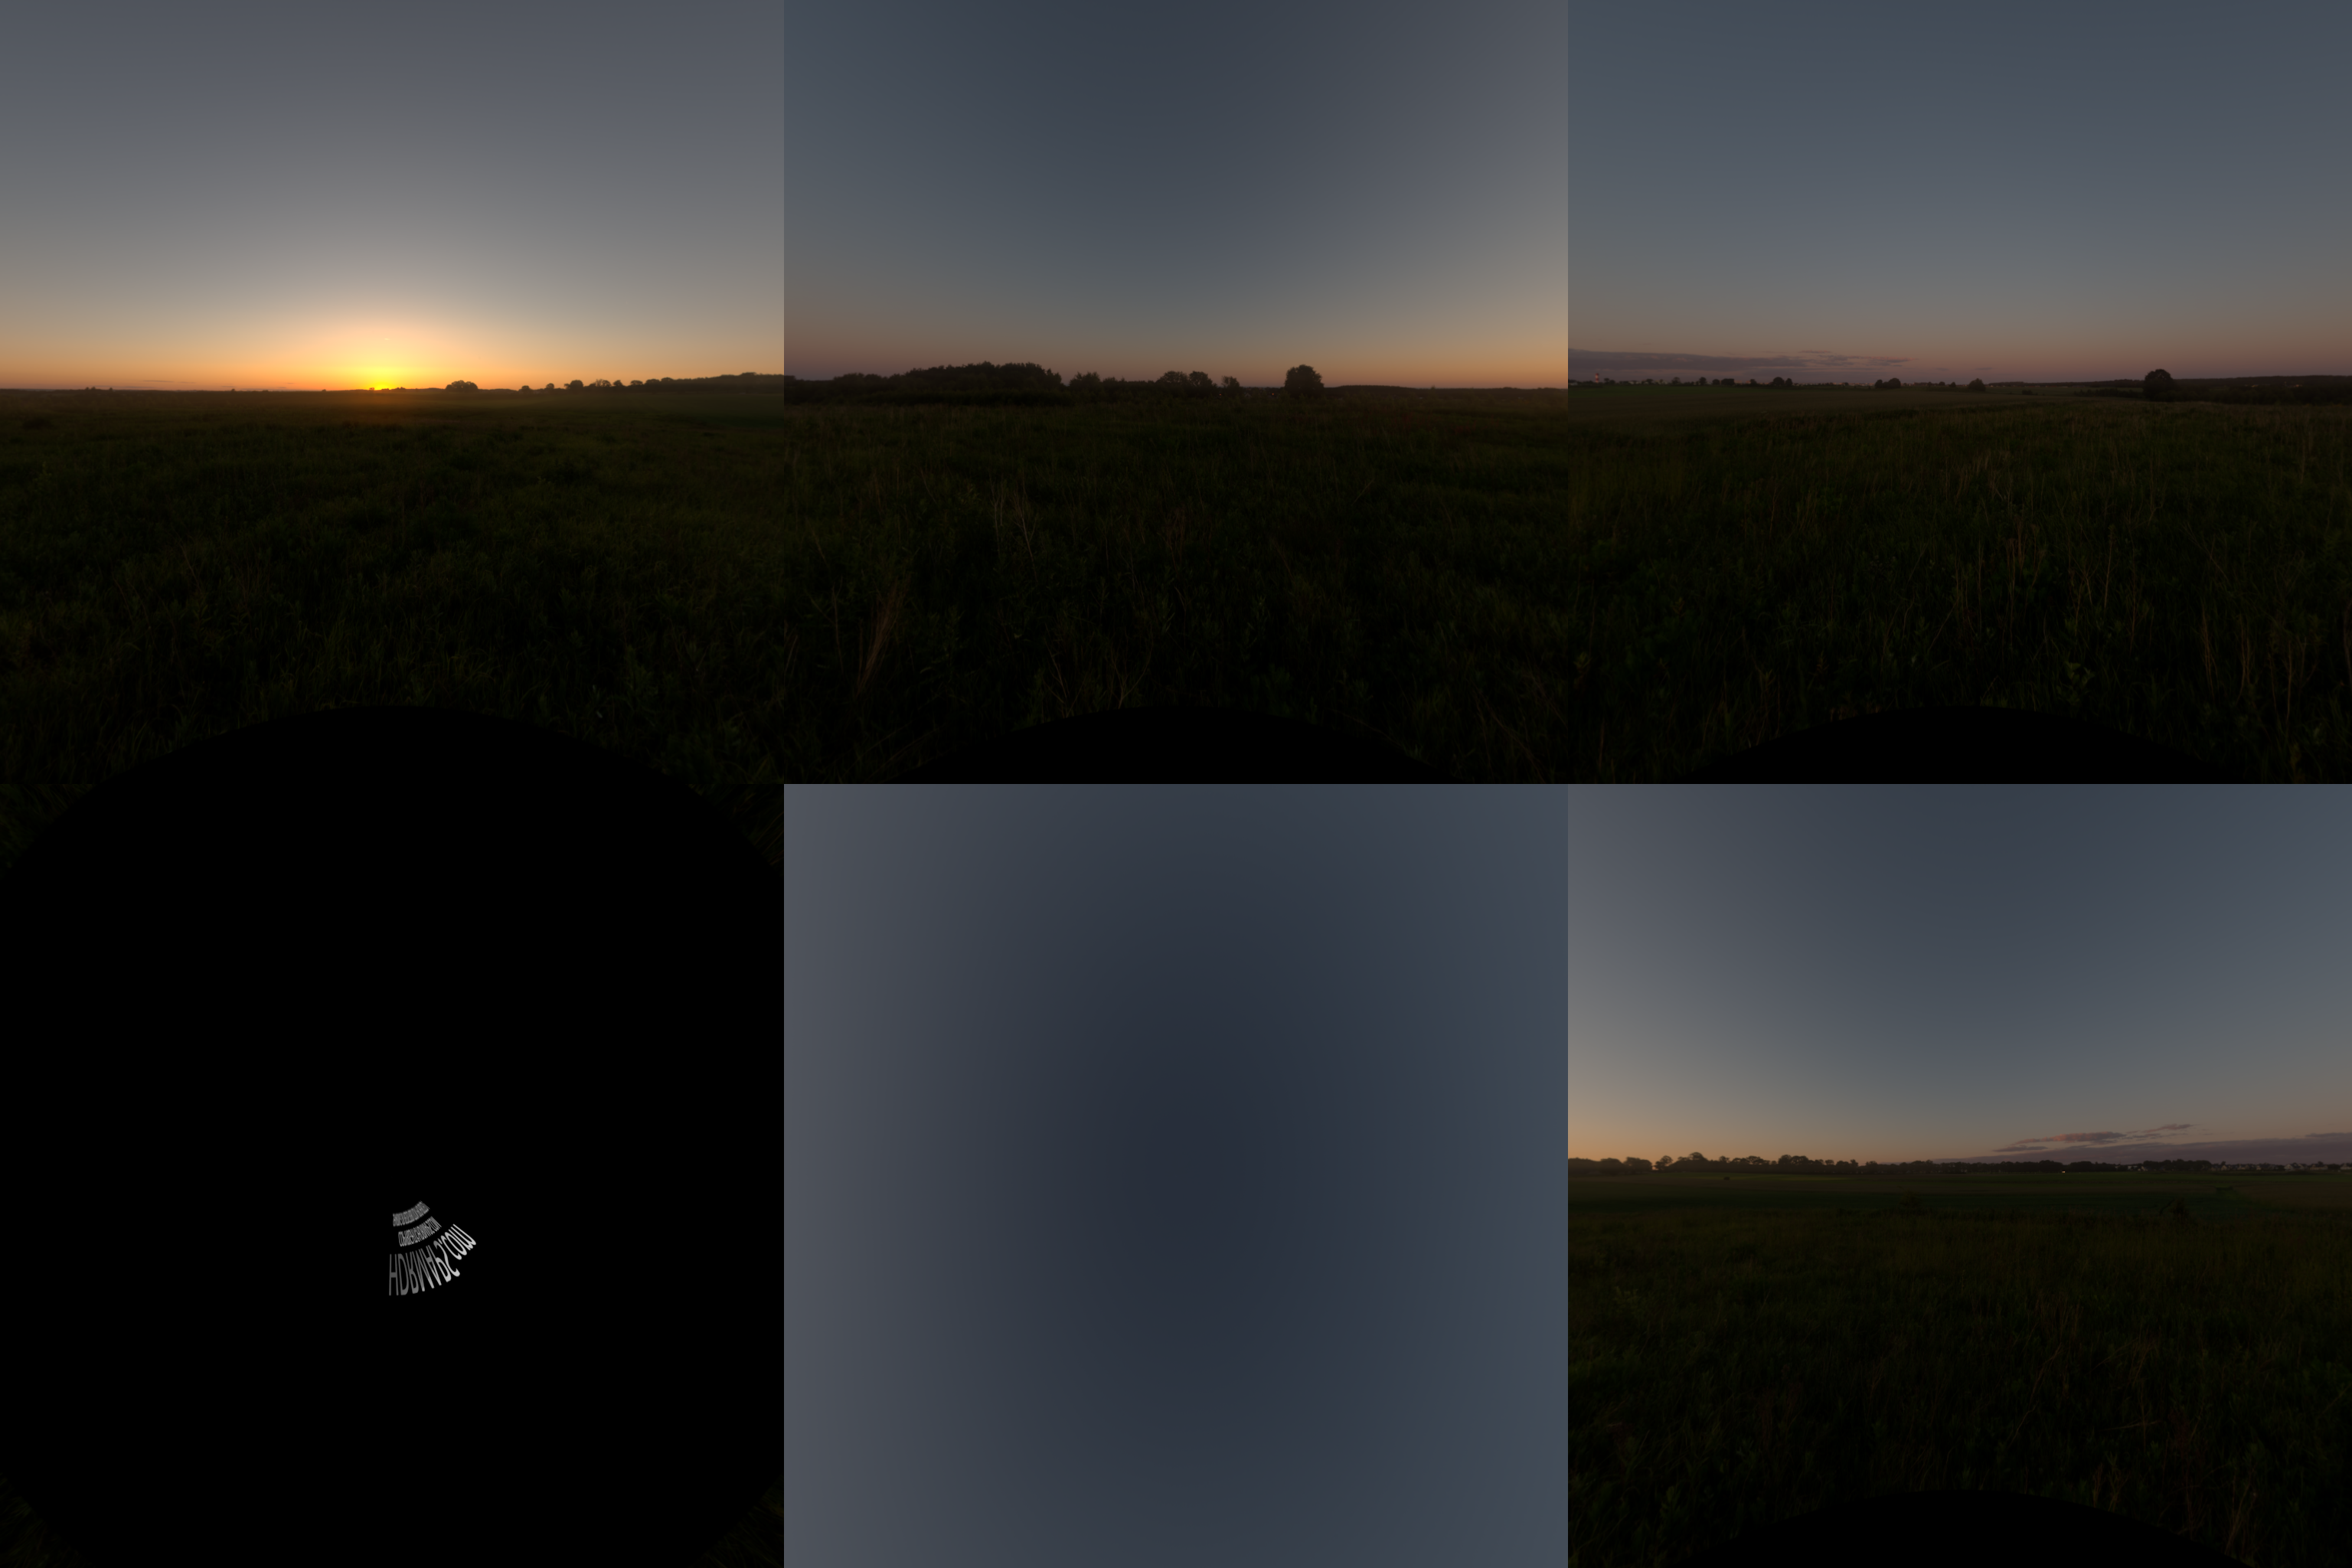
\includegraphics[width=0.4\textwidth]{pictures/EnvMap_cube_1024.png}
\caption{Source: https://hdrmaps.com }
\end{figure}

\vfill

\begin{lstlisting}[caption={Implementing the Skybox}][H!]
SkyBackgroundUnrecPtr loadBackground(Resolutions skyboxResolution) {
   
 std::string bgImageFilePath = Path_to_Skybox_image;

 ImageUnrecPtr mainImage = ImageFileHandler::the()->read(bgImageFilePath.c_str());

 /**
 * Create empty images as destinations for subimage */
 ImageUnrecPtr imgFront = ImageBase::create();
 ImageUnrecPtr imgBack = ImageBase::create();
 ImageUnrecPtr imgLeft = ImageBase::create();
 ImageUnrecPtr imgRight = ImageBase::create();
 ImageUnrecPtr imgTop = ImageBase::create();
 ImageUnrecPtr imgBottom = ImageBase::create();

 /**
  * Easier to change Skybox Images by croping them out
  * at runtime directly from the CubeMap Image exported from Blender
  *
  * Blender exports the environment maps in the format:
  *
  * Left   | Back | Right
  * Bottom | Top  | Front
  *
  * While subImage reads 
  * - offX from left to right
  * - offY from bottom to top */
 mainImage->subImage(2 * res, 0  , 0, 
   res, res, 1, 
   imgFront);
 mainImage->subImage(res , res, 0, 
   res, res, 1,
    imgBack);
 mainImage->subImage(0  , res, 0, 
   res, res, 1, 
   imgLeft);
 mainImage->subImage(2 * res, res, 
   0, res, res, 1, 
   imgRight);
 mainImage->subImage(res, 0  , 0, 
   res, res, 1, 
   imgTop);
 mainImage->subImage(0 , 0  , 0, 
   res, res, 1, 
   imgBottom);

    /**
     * Create Textures and set image to cropped images */
    TextureObjChunkUnrecPtr texFront = TextureObjChunk::create();
    texFront->setImage(imgFront);

    TextureObjChunkUnrecPtr texBack = TextureObjChunk::create();
    texBack->setImage(imgBack);

    TextureObjChunkUnrecPtr texLeft = TextureObjChunk::create();
    texLeft->setImage(imgLeft);

    TextureObjChunkUnrecPtr texRight = TextureObjChunk::create();
    texRight->setImage(imgRight);

    TextureObjChunkUnrecPtr texTop = TextureObjChunk::create();
    texTop->setImage(imgTop);

    TextureObjChunkUnrecPtr texBottom = TextureObjChunk::create();
    texBottom->setImage(imgBottom);

    /**
     * Create Skybox and set textures */
    SkyBackgroundUnrecPtr skyBG = SkyBackground::create();
    skyBG->setFrontTexture(texFront);
    skyBG->setBackTexture(texBack);
    skyBG->setLeftTexture(texLeft);
    skyBG->setRightTexture(texRight);
    skyBG->setTopTexture(texTop);
    skyBG->setBottomTexture(texBottom);

    return skyBG;
}

\end{lstlisting}

\subsection{Animations}

While the \emph{Lerp} and the \emph{FracTime} was easy to implement in c++, for the \emph{Coroutines} had to be found another solution. To make things easy an animation holder was implemented, controlling all animations of the scene in one place.

\begin{lstlisting}[breaklines=true]
void Scene::update(OSG::Time dTime) {
 _animations.animate(dTime);
}
\end{lstlisting}

The framework which was implemented uses two main animation classes \lq\lq{}ParallelAnimation\rq\rq{} and \lq\lq{}SequentialAnimation\rq\rq{} defining as the name lets guess already whether contained animations shall be performed simultaneously or sequentially. So it\rq{}s easy to guess that the Scene::\_animations is a ParallelAnimation animating all contained animations at the same time.
\begin{lstlisting}[breaklines=true, caption={ParallelAnimation::animate}]
void ParallelAnimation::animate(OSG::Time dTime) {
 for (auto animation : _animations) {
  animation->animate(dTime);
 }
 removeStoppedAnimations();
 if (_stopIfNoAnimations && _animations.empty()) {
  stop();
 }
}
\end{lstlisting}

\begin{lstlisting}[breaklines=true, caption={SequentialAnimation::animate}]
void SequentialAnimation::animate(OSG::Time dTime) {
 if (_stopIfNoAnimations && _animations.empty()) {
  stop();
 } else {
  _animations.front()->animate(dTime);
  if (_animations.front()->isStopped()) {
   _animations.pop();
   if (_stopIfNoAnimations && _animations.empty()) {
    stop();
   }
  }
 }
}
\end{lstlisting}

Then there are some animation wrappers like \lq\lq{}EaseInAnimation\rq\rq{}, \lq\lq{}EaseOutAnimation\rq\rq{} and \lq\lq{}BezierAnimation\rq\rq{} allowing to implement completely ease controlled animations and even a forward-backwards animation as seen in the example below:
\begin{lstlisting}[breaklines=true, caption={BezierAnimation::animate}]
void BezierAnimation::animateFracTime(OSG::Time fracTime) {
 _animation->animate(_bezier.atPercentage(fracTime).y());
}
\end{lstlisting}

Finally there are the actual animation performing the before mentioned Lerp on Vectors \lq\lq{}TranslationAnimation\rq\rq{} and \lq\lq{}ScaleAnimation\rq\rq{} as seen in the example below:
\begin{lstlisting}[breaklines=true, caption={TranslattionAnimation::animate}]
void TranslationAnimation::animateFracTime(OSG::Time fracTime) {
 Vec3f _movement = _destination - _start;
 _trans->setTranslation(_start + _movement * fracTime);
}
\end{lstlisting}

\subsection{Effects}
Based on this animations framework the effects and user feedback was implemented using for example a TranslationAnimation and a ScaleAnimation wrapped in a ParallelAnimation with repetition enabled:
\begin{lstlisting}[breaklines=true, caption={BubbleAnimationsNode::animate}]
void BubbleAnimationsNode::addAnimations() {
 for (const auto &data : _bubbleDatas) {
  _animations.add(std::shared_ptr<Animation>(
   new ParallelAnimation{
    std::shared_ptr<Animation>(
     new TranslationAnimation(
      data.transformation,
      OSG::Vec3f(0, 1, 0),
      3 * data.data, true)),

    std::shared_ptr<Animation>(
     new ScaleAnimation(
      data.transformation,
      OSG::Vec3f(0, 0, 0),
      3 * data.data, true))
     }
  ));
 }
}
\end{lstlisting}
